\documentclass[../main]{subfiles}

\questiontrue
\solutiontrue

\begin{document}
    \ifquestion
    
    \section{Orbit Control}
	
A space probe with mass \( m_0 \) is in a circular orbit with velocity \( v_0 \) around a homogeneous spherical planet without an atmosphere, with mass $ M $ ($ M \gg m_0 $) and radius \( R \), at a distance \( \alpha R \) ($ \alpha > 1 $) from the center of the planet. The team of astronauts, called *Vinhedeiros*, wants to perform an elliptical orbit as close as possible to the planet (without causing collisions, of course). To achieve this, the engines will be activated, releasing propellant at a velocity \( u \) relative to the engines. It is known that the engine releases propellant at a constant rate equal to \( K \).

\ut{a} How long should the engine be programmed to remain active? Hint: Although the propellant release is not instantaneous, consider that this time is much shorter than the orbital period, so intermediate changes can be disregarded.

\ut{b} What will this time be for a soft landing on the planet? Use the same considerations.
    
	\clearpage
    
    \fi
    
    \ifsolution
    
    \section{Orbit Control}
	
	\ut{a} The first step to solve the problem is to better visualize the orbits and to identify the transfers that need to occur, like shown in the Figure \ref{fig:elipsiiiii}:

    \begin{figure}[htpb]
        \centering
        

\tikzset{every picture/.style={line width=0.75pt}} %set default line width to 0.75pt        

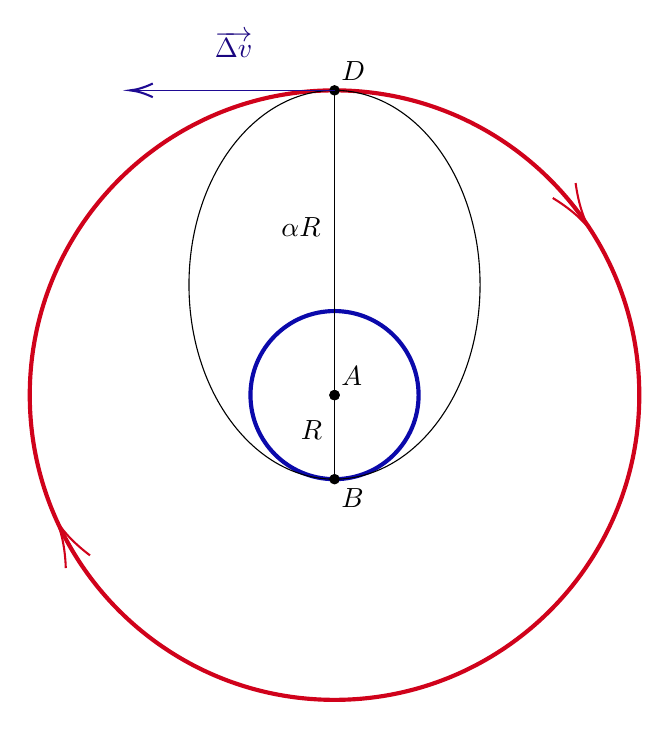
\begin{tikzpicture}[x=0.75pt,y=0.75pt,yscale=-1,xscale=1]
%uncomment if require: \path (0,542); %set diagram left start at 0, and has height of 542

%Shape: Circle [id:dp6173545101257163] 
\draw  [color={rgb, 255:red, 11; green, 9; blue, 171 }  ,draw opacity=1 ][line width=1.5]  (295.67,353.51) .. controls (295.67,331.14) and (313.8,313.01) .. (336.17,313.01) .. controls (358.53,313.01) and (376.67,331.14) .. (376.67,353.51) .. controls (376.67,375.88) and (358.53,394.01) .. (336.17,394.01) .. controls (313.8,394.01) and (295.67,375.88) .. (295.67,353.51) -- cycle ;
%Shape: Circle [id:dp015889685031721612] 
\draw  [color={rgb, 255:red, 208; green, 2; blue, 27 }  ,draw opacity=1 ][line width=1.5]  (189.33,353.51) .. controls (189.33,272.42) and (255.07,206.68) .. (336.17,206.68) .. controls (417.26,206.68) and (483,272.42) .. (483,353.51) .. controls (483,434.6) and (417.26,500.34) .. (336.17,500.34) .. controls (255.07,500.34) and (189.33,434.6) .. (189.33,353.51) -- cycle ;
%Shape: Ellipse [id:dp2422523805926604] 
\draw   (336.17,206.68) .. controls (374.9,206.68) and (406.29,248.61) .. (406.29,300.34) .. controls (406.29,352.07) and (374.9,394.01) .. (336.17,394.01) .. controls (297.44,394.01) and (266.04,352.07) .. (266.04,300.34) .. controls (266.04,248.61) and (297.44,206.68) .. (336.17,206.68) -- cycle ;
%Straight Lines [id:da9056607434107695] 
\draw    (336.17,353.51) -- (336.17,394.01) ;
\draw [shift={(336.17,394.01)}, rotate = 90] [color={rgb, 255:red, 0; green, 0; blue, 0 }  ][fill={rgb, 255:red, 0; green, 0; blue, 0 }  ][line width=0.75]      (0, 0) circle [x radius= 2.01, y radius= 2.01]   ;
\draw [shift={(336.17,353.51)}, rotate = 90] [color={rgb, 255:red, 0; green, 0; blue, 0 }  ][fill={rgb, 255:red, 0; green, 0; blue, 0 }  ][line width=0.75]      (0, 0) circle [x radius= 2.01, y radius= 2.01]   ;
%Straight Lines [id:da46758598270689533] 
\draw    (336.17,206.68) -- (336.17,353.51) ;
\draw [shift={(336.17,353.51)}, rotate = 90] [color={rgb, 255:red, 0; green, 0; blue, 0 }  ][fill={rgb, 255:red, 0; green, 0; blue, 0 }  ][line width=0.75]      (0, 0) circle [x radius= 2.01, y radius= 2.01]   ;
\draw [shift={(336.17,206.68)}, rotate = 90] [color={rgb, 255:red, 0; green, 0; blue, 0 }  ][fill={rgb, 255:red, 0; green, 0; blue, 0 }  ][line width=0.75]      (0, 0) circle [x radius= 2.01, y radius= 2.01]   ;
%Straight Lines [id:da5578682461981412] 
\draw [color={rgb, 255:red, 208; green, 2; blue, 27 }  ,draw opacity=1 ]   (454.79,267.11) -- (457.69,271.55) ;
\draw [shift={(458.79,273.22)}, rotate = 236.77] [color={rgb, 255:red, 208; green, 2; blue, 27 }  ,draw opacity=1 ][line width=0.75]    (21.86,-6.58) .. controls (13.9,-2.79) and (6.61,-0.6) .. (0,0) .. controls (6.61,0.6) and (13.9,2.79) .. (21.86,6.58)   ;
%Straight Lines [id:da5731048394454692] 
\draw [color={rgb, 255:red, 208; green, 2; blue, 27 }  ,draw opacity=1 ]   (206,421.25) -- (203.35,416.16) ;
\draw [shift={(202.43,414.39)}, rotate = 62.49] [color={rgb, 255:red, 208; green, 2; blue, 27 }  ,draw opacity=1 ][line width=0.75]    (21.86,-6.58) .. controls (13.9,-2.79) and (6.61,-0.6) .. (0,0) .. controls (6.61,0.6) and (13.9,2.79) .. (21.86,6.58)   ;
%Straight Lines [id:da7752817797347507] 
\draw [color={rgb, 255:red, 30; green, 10; blue, 147 }  ,draw opacity=1 ]   (336.17,206.68) -- (239.67,206.68) ;
\draw [shift={(237.67,206.68)}, rotate = 360] [color={rgb, 255:red, 30; green, 10; blue, 147 }  ,draw opacity=1 ][line width=0.75]    (10.93,-3.29) .. controls (6.95,-1.4) and (3.31,-0.3) .. (0,0) .. controls (3.31,0.3) and (6.95,1.4) .. (10.93,3.29)   ;

% Text Node
\draw (318.67,364.74) node [anchor=north west][inner sep=0.75pt]    {$R$};
% Text Node
\draw (309.33,266.74) node [anchor=north west][inner sep=0.75pt]    {$\alpha R$};
% Text Node
\draw (338.17,397.41) node [anchor=north west][inner sep=0.75pt]    {$B$};
% Text Node
\draw (338.17,350.11) node [anchor=south west] [inner sep=0.75pt]    {$A$};
% Text Node
\draw (338.17,203.28) node [anchor=south west] [inner sep=0.75pt]    {$D$};
% Text Node
\draw (277.24,176.75) node [anchor=north west][inner sep=0.75pt]  [color={rgb, 255:red, 26; green, 6; blue, 128 }  ,opacity=1 ]  {$\overrightarrow{\Delta v}$};


\end{tikzpicture}
        \caption{Transfer orbits for the given situation}
        \label{fig:elipsiiiii}
    \end{figure}	


	
Consider the initial orbit as the largest circle, with the planet represented by the colored circumference, and the intermediate ellipse as the transfer orbit.

Note that since we want the spacecraft to pass as close as possible to the planet's surface without colliding, we aim for the periapsis of the elliptical orbit to approach the planet's radius as closely as possible. Thus, in the limiting case:  
\[2a = R + \alpha R = (1 + \alpha)R\]
Therefore, we have:  
\[a = \frac{1 + \alpha}{2}R\]
Calculating the \(\Delta v\) between the two orbits (from circular to elliptical): 

\[\Delta v = \sqrt{GM\left(\frac{2}{r} - \frac{1}{a}\right)} - \sqrt{GM\frac{1}{r}}\]
\[\Delta v = \sqrt{GM\left(\frac{2}{\alpha R} - \frac{2}{(1 + \alpha)R}\right)} - \sqrt{\frac{GM}{\alpha R}}\]
\[\therefore \Delta v = \sqrt{\frac{GM}{(1 + \alpha)\alpha R}}(\sqrt{2} - \sqrt{1 + \alpha})\]

Note that since \(\alpha > 1\), we have \(1 + \alpha > 2\), thus \(\Delta v < 0\), as expected.

Now we can relate the time the engines remain active with the \(\Delta v\) required for the transfer.  
Using the rocket equation:  

\[|\Delta v| = u \ln{\frac{m_0}{m_f}}\]

Since mass is ejected at a rate \(K\), we can express the final mass of the rocket as \(m_f = m_0 - K\Delta t\). Applying and rearranging:  

\[\frac{m_0}{K}\left(1 - e^{-\frac{|\Delta v|}{u}}\right) = \Delta t\]

Finalizing:  

\[\Delta t = \frac{m_0}{K}\left(1 - e^{\frac{1}{u}\sqrt{\frac{GM}{(1 + \alpha)\alpha R}}(\sqrt{2} - \sqrt{1 + \alpha})}\right)\]

\ut{b} In this case, it is enough to stop the spacecraft to achieve a soft landing, meaning \(\Delta v = v\). For this situation:  

\[v = \sqrt{GM\left(\frac{2}{R} + \frac{2}{(\alpha + 1)R}\right)}\]

\[v = \sqrt{\frac{2GM(\alpha + 2)}{(\alpha + 1)R}}\]

Thus, using the formula found in the previous item:  

	\[\Delta t = \frac{m_0}{K}\left(1-e^{-\sqrt{\frac{2GM(\alpha+2)}{u^2R(\alpha+1)}}}\right)\]
	
	
	
	
	\clearpage
    
    
    \fi
\end{document}
